% !TEX program = pdflatex
% Requiere correr antes:  python3 analisis_datos.py
% Compilar: pdflatex analisis_datos && bibtex analisis_datos && pdflatex analisis_datos && pdflatex analisis_datos
\documentclass[11pt,a4paper,parskip=half]{scrartcl}
% ============================================================
% estilo.tex — preámbulo compartido por los tres documentos
% Se incluye con % ============================================================
% estilo.tex — preámbulo compartido por los tres documentos
% Se incluye con % ============================================================
% estilo.tex — preámbulo compartido por los tres documentos
% Se incluye con \input{estilo} después de \documentclass
% ============================================================

\usepackage[utf8]{inputenc}
\usepackage[T1]{fontenc}
\usepackage{lmodern}
\usepackage[spanish]{babel}

\usepackage[a4paper,margin=2.5cm]{geometry}
\usepackage{microtype}
\usepackage{enumitem}
\usepackage{booktabs}
\usepackage{longtable}
\usepackage{tabularx}
\usepackage{array}
\usepackage{colortbl}

\usepackage{xcolor}
\definecolor{ink}{RGB}{0,62,92}           % azul principal
\definecolor{inklight}{RGB}{92,132,153}   % azul apagado
\definecolor{rulegray}{RGB}{205,214,219}  % líneas divisorias
\definecolor{critred}{RGB}{158,38,32}     % prioridad crítica
\definecolor{amber}{RGB}{176,98,16}       % prioridad alta
\definecolor{slate}{RGB}{104,112,118}     % prioridad media
\definecolor{headrow}{RGB}{0,62,92}       % encabezado de tabla
\definecolor{softrow}{RGB}{242,246,248}   % fila alterna

\usepackage{natbib}   % debe cargarse antes que hyperref
\usepackage[colorlinks=true,linkcolor=ink,citecolor=inklight,urlcolor=inklight]{hyperref}

% ---------- títulos ----------
\addtokomafont{title}{\color{ink}\sffamily}
\addtokomafont{author}{\color{slate}\normalsize}
\addtokomafont{date}{\color{slate}\normalsize}
\addtokomafont{disposition}{\color{ink}\sffamily}
\setkomafont{section}{\color{ink}\sffamily\large\bfseries}
\setkomafont{subsection}{\color{ink}\sffamily\normalsize\bfseries}

% ---------- lista de campos alineada (reemplaza las cajas) ----------
\newlist{campos}{description}{1}
\setlist[campos]{
  labelwidth=2.9cm,
  leftmargin=3.2cm,
  labelsep=0.3cm,
  align=left,
  font=\normalfont\sffamily\bfseries\small\color{ink},
  itemsep=2.5pt,
  topsep=4pt,
  parsep=0pt,
  before=\small
}

% ---------- etiqueta de prioridad ----------
\newcommand{\prio}[2]{%
  {\setlength{\fboxsep}{3pt}%
   \colorbox{#1}{\textcolor{white}{\sffamily\bfseries\scriptsize\strut\,#2\,}}}%
}
\newcommand{\critica}{\prio{critred}{CRÍTICA}}
\newcommand{\alta}{\prio{amber}{ALTA}}
\newcommand{\media}{\prio{slate}{MEDIA}}

\newsavebox{\cajaetiqueta}
\newlength{\sepetiqueta}\setlength{\sepetiqueta}{10pt}

% ---------- encabezado de una entrada (pregunta o ficha) ----------
% #1 = clave corta (Q1 / P-04)   #2 = título   #3 = etiqueta derecha
\newcommand{\entrada}[3]{%
  \par\addvspace{14pt}%
  \noindent{\color{rulegray}\rule{\linewidth}{0.6pt}}%
  \par\addvspace{5pt}%
  \noindent
  \sbox\cajaetiqueta{#3}%
  \begin{minipage}[t]{\dimexpr\linewidth-\wd\cajaetiqueta-\sepetiqueta\relax}
    \raggedright\sffamily\bfseries\color{ink}#1\,\textcolor{rulegray}{\textbar}\, #2
  \end{minipage}\hspace{\sepetiqueta}\usebox\cajaetiqueta%
  \par\addvspace{3pt}%
}

% variante sin clave a la izquierda (para fichas bibliográficas)
\newcommand{\entradasimple}[2]{%
  \par\addvspace{14pt}%
  \noindent{\color{rulegray}\rule{\linewidth}{0.6pt}}%
  \par\addvspace{5pt}%
  \noindent
  \sbox\cajaetiqueta{#2}%
  \begin{minipage}[t]{\dimexpr\linewidth-\wd\cajaetiqueta-\sepetiqueta\relax}
    \raggedright\sffamily\bfseries\color{ink}#1
  \end{minipage}\hspace{\sepetiqueta}\usebox\cajaetiqueta%
  \par\addvspace{3pt}%
}

% permite cortar nombres largos de campo en \texttt sin salirse del margen
\newcommand{\campoTT}[2]{\texttt{#1\_}\allowbreak\texttt{#2}}

% ---------- nota destacada, sin caja pesada ----------
\newenvironment{nota}{%
  \par\addvspace{8pt}\small
  \begin{list}{}{%
    \setlength{\leftmargin}{10pt}\setlength{\rightmargin}{0pt}
    \setlength{\labelwidth}{0pt}\setlength{\itemindent}{0pt}
    \setlength{\listparindent}{0pt}}
  \item[]\color{black}%
}{%
  \end{list}\addvspace{6pt}%
}

% ---------- tablas ----------
\newcolumntype{L}[1]{>{\raggedright\arraybackslash}p{#1}}
\newcommand{\thead}[1]{\textcolor{white}{\sffamily\bfseries\small #1}}

\renewcommand{\arraystretch}{1.25}
\setlength{\tabcolsep}{5pt}
 después de \documentclass
% ============================================================

\usepackage[utf8]{inputenc}
\usepackage[T1]{fontenc}
\usepackage{lmodern}
\usepackage[spanish]{babel}

\usepackage[a4paper,margin=2.5cm]{geometry}
\usepackage{microtype}
\usepackage{enumitem}
\usepackage{booktabs}
\usepackage{longtable}
\usepackage{tabularx}
\usepackage{array}
\usepackage{colortbl}

\usepackage{xcolor}
\definecolor{ink}{RGB}{0,62,92}           % azul principal
\definecolor{inklight}{RGB}{92,132,153}   % azul apagado
\definecolor{rulegray}{RGB}{205,214,219}  % líneas divisorias
\definecolor{critred}{RGB}{158,38,32}     % prioridad crítica
\definecolor{amber}{RGB}{176,98,16}       % prioridad alta
\definecolor{slate}{RGB}{104,112,118}     % prioridad media
\definecolor{headrow}{RGB}{0,62,92}       % encabezado de tabla
\definecolor{softrow}{RGB}{242,246,248}   % fila alterna

\usepackage{natbib}   % debe cargarse antes que hyperref
\usepackage[colorlinks=true,linkcolor=ink,citecolor=inklight,urlcolor=inklight]{hyperref}

% ---------- títulos ----------
\addtokomafont{title}{\color{ink}\sffamily}
\addtokomafont{author}{\color{slate}\normalsize}
\addtokomafont{date}{\color{slate}\normalsize}
\addtokomafont{disposition}{\color{ink}\sffamily}
\setkomafont{section}{\color{ink}\sffamily\large\bfseries}
\setkomafont{subsection}{\color{ink}\sffamily\normalsize\bfseries}

% ---------- lista de campos alineada (reemplaza las cajas) ----------
\newlist{campos}{description}{1}
\setlist[campos]{
  labelwidth=2.9cm,
  leftmargin=3.2cm,
  labelsep=0.3cm,
  align=left,
  font=\normalfont\sffamily\bfseries\small\color{ink},
  itemsep=2.5pt,
  topsep=4pt,
  parsep=0pt,
  before=\small
}

% ---------- etiqueta de prioridad ----------
\newcommand{\prio}[2]{%
  {\setlength{\fboxsep}{3pt}%
   \colorbox{#1}{\textcolor{white}{\sffamily\bfseries\scriptsize\strut\,#2\,}}}%
}
\newcommand{\critica}{\prio{critred}{CRÍTICA}}
\newcommand{\alta}{\prio{amber}{ALTA}}
\newcommand{\media}{\prio{slate}{MEDIA}}

\newsavebox{\cajaetiqueta}
\newlength{\sepetiqueta}\setlength{\sepetiqueta}{10pt}

% ---------- encabezado de una entrada (pregunta o ficha) ----------
% #1 = clave corta (Q1 / P-04)   #2 = título   #3 = etiqueta derecha
\newcommand{\entrada}[3]{%
  \par\addvspace{14pt}%
  \noindent{\color{rulegray}\rule{\linewidth}{0.6pt}}%
  \par\addvspace{5pt}%
  \noindent
  \sbox\cajaetiqueta{#3}%
  \begin{minipage}[t]{\dimexpr\linewidth-\wd\cajaetiqueta-\sepetiqueta\relax}
    \raggedright\sffamily\bfseries\color{ink}#1\,\textcolor{rulegray}{\textbar}\, #2
  \end{minipage}\hspace{\sepetiqueta}\usebox\cajaetiqueta%
  \par\addvspace{3pt}%
}

% variante sin clave a la izquierda (para fichas bibliográficas)
\newcommand{\entradasimple}[2]{%
  \par\addvspace{14pt}%
  \noindent{\color{rulegray}\rule{\linewidth}{0.6pt}}%
  \par\addvspace{5pt}%
  \noindent
  \sbox\cajaetiqueta{#2}%
  \begin{minipage}[t]{\dimexpr\linewidth-\wd\cajaetiqueta-\sepetiqueta\relax}
    \raggedright\sffamily\bfseries\color{ink}#1
  \end{minipage}\hspace{\sepetiqueta}\usebox\cajaetiqueta%
  \par\addvspace{3pt}%
}

% permite cortar nombres largos de campo en \texttt sin salirse del margen
\newcommand{\campoTT}[2]{\texttt{#1\_}\allowbreak\texttt{#2}}

% ---------- nota destacada, sin caja pesada ----------
\newenvironment{nota}{%
  \par\addvspace{8pt}\small
  \begin{list}{}{%
    \setlength{\leftmargin}{10pt}\setlength{\rightmargin}{0pt}
    \setlength{\labelwidth}{0pt}\setlength{\itemindent}{0pt}
    \setlength{\listparindent}{0pt}}
  \item[]\color{black}%
}{%
  \end{list}\addvspace{6pt}%
}

% ---------- tablas ----------
\newcolumntype{L}[1]{>{\raggedright\arraybackslash}p{#1}}
\newcommand{\thead}[1]{\textcolor{white}{\sffamily\bfseries\small #1}}

\renewcommand{\arraystretch}{1.25}
\setlength{\tabcolsep}{5pt}
 después de \documentclass
% ============================================================

\usepackage[utf8]{inputenc}
\usepackage[T1]{fontenc}
\usepackage{lmodern}
\usepackage[spanish]{babel}

\usepackage[a4paper,margin=2.5cm]{geometry}
\usepackage{microtype}
\usepackage{enumitem}
\usepackage{booktabs}
\usepackage{longtable}
\usepackage{tabularx}
\usepackage{array}
\usepackage{colortbl}

\usepackage{xcolor}
\definecolor{ink}{RGB}{0,62,92}           % azul principal
\definecolor{inklight}{RGB}{92,132,153}   % azul apagado
\definecolor{rulegray}{RGB}{205,214,219}  % líneas divisorias
\definecolor{critred}{RGB}{158,38,32}     % prioridad crítica
\definecolor{amber}{RGB}{176,98,16}       % prioridad alta
\definecolor{slate}{RGB}{104,112,118}     % prioridad media
\definecolor{headrow}{RGB}{0,62,92}       % encabezado de tabla
\definecolor{softrow}{RGB}{242,246,248}   % fila alterna

\usepackage{natbib}   % debe cargarse antes que hyperref
\usepackage[colorlinks=true,linkcolor=ink,citecolor=inklight,urlcolor=inklight]{hyperref}

% ---------- títulos ----------
\addtokomafont{title}{\color{ink}\sffamily}
\addtokomafont{author}{\color{slate}\normalsize}
\addtokomafont{date}{\color{slate}\normalsize}
\addtokomafont{disposition}{\color{ink}\sffamily}
\setkomafont{section}{\color{ink}\sffamily\large\bfseries}
\setkomafont{subsection}{\color{ink}\sffamily\normalsize\bfseries}

% ---------- lista de campos alineada (reemplaza las cajas) ----------
\newlist{campos}{description}{1}
\setlist[campos]{
  labelwidth=2.9cm,
  leftmargin=3.2cm,
  labelsep=0.3cm,
  align=left,
  font=\normalfont\sffamily\bfseries\small\color{ink},
  itemsep=2.5pt,
  topsep=4pt,
  parsep=0pt,
  before=\small
}

% ---------- etiqueta de prioridad ----------
\newcommand{\prio}[2]{%
  {\setlength{\fboxsep}{3pt}%
   \colorbox{#1}{\textcolor{white}{\sffamily\bfseries\scriptsize\strut\,#2\,}}}%
}
\newcommand{\critica}{\prio{critred}{CRÍTICA}}
\newcommand{\alta}{\prio{amber}{ALTA}}
\newcommand{\media}{\prio{slate}{MEDIA}}

\newsavebox{\cajaetiqueta}
\newlength{\sepetiqueta}\setlength{\sepetiqueta}{10pt}

% ---------- encabezado de una entrada (pregunta o ficha) ----------
% #1 = clave corta (Q1 / P-04)   #2 = título   #3 = etiqueta derecha
\newcommand{\entrada}[3]{%
  \par\addvspace{14pt}%
  \noindent{\color{rulegray}\rule{\linewidth}{0.6pt}}%
  \par\addvspace{5pt}%
  \noindent
  \sbox\cajaetiqueta{#3}%
  \begin{minipage}[t]{\dimexpr\linewidth-\wd\cajaetiqueta-\sepetiqueta\relax}
    \raggedright\sffamily\bfseries\color{ink}#1\,\textcolor{rulegray}{\textbar}\, #2
  \end{minipage}\hspace{\sepetiqueta}\usebox\cajaetiqueta%
  \par\addvspace{3pt}%
}

% variante sin clave a la izquierda (para fichas bibliográficas)
\newcommand{\entradasimple}[2]{%
  \par\addvspace{14pt}%
  \noindent{\color{rulegray}\rule{\linewidth}{0.6pt}}%
  \par\addvspace{5pt}%
  \noindent
  \sbox\cajaetiqueta{#2}%
  \begin{minipage}[t]{\dimexpr\linewidth-\wd\cajaetiqueta-\sepetiqueta\relax}
    \raggedright\sffamily\bfseries\color{ink}#1
  \end{minipage}\hspace{\sepetiqueta}\usebox\cajaetiqueta%
  \par\addvspace{3pt}%
}

% permite cortar nombres largos de campo en \texttt sin salirse del margen
\newcommand{\campoTT}[2]{\texttt{#1\_}\allowbreak\texttt{#2}}

% ---------- nota destacada, sin caja pesada ----------
\newenvironment{nota}{%
  \par\addvspace{8pt}\small
  \begin{list}{}{%
    \setlength{\leftmargin}{10pt}\setlength{\rightmargin}{0pt}
    \setlength{\labelwidth}{0pt}\setlength{\itemindent}{0pt}
    \setlength{\listparindent}{0pt}}
  \item[]\color{black}%
}{%
  \end{list}\addvspace{6pt}%
}

% ---------- tablas ----------
\newcolumntype{L}[1]{>{\raggedright\arraybackslash}p{#1}}
\newcommand{\thead}[1]{\textcolor{white}{\sffamily\bfseries\small #1}}

\renewcommand{\arraystretch}{1.25}
\setlength{\tabcolsep}{5pt}

\usepackage{graphicx}
\bibliographystyle{apalike}

% Todas las cifras de este documento las genera analisis_datos.py.
% Ninguna está escrita a mano.
% Generado por analisis_datos.py -- NO editar a mano.
% Volver a generar con:  python3 analisis_datos.py

\newcommand{\servicioDia}{L}
\newcommand{\registrosViaje}{6.629}
\newcommand{\viajesDelDia}{7.917}
\newcommand{\viajesNoBus}{1.288}
\newcommand{\pctNoBus}{16{,}3}
\newcommand{\corridasReales}{64.603}
\newcommand{\factorFrecuencia}{9{,}7}
\newcommand{\pctFrecuencia}{100{,}0}
\newcommand{\duracionMedia}{73{,}8}
\newcommand{\duracionMediana}{67{,}5}
\newcommand{\duracionMin}{8}
\newcommand{\duracionMax}{198}
\newcommand{\distanciaMedia}{20{,}6}
\newcommand{\distanciaMediana}{19{,}5}
\newcommand{\distanciaMin}{2{,}3}
\newcommand{\distanciaMax}{57{,}6}
\newcommand{\kmTotales}{1.346.022}
\newcommand{\horasBus}{84.483}
\newcommand{\consumoImplicito}{1{,}40}
\newcommand{\consumoReal}{1{,}006}
\newcommand{\energiaImplicita}{1{,}88}
\newcommand{\energiaReal}{1{,}35}
\newcommand{\autonomiaUtil}{225}
\newcommand{\picoSimultaneo}{6.603}
\newcommand{\horaPico}{08:00}
\newcommand{\flotaDeclarada}{1.200}
\newcommand{\cuposTotales}{700}
\newcommand{\numElectroterminales}{5}
\newcommand{\ratioFlota}{5{,}5}
\newcommand{\ratioCupos}{9{,}4}
\newcommand{\flotaRealRED}{6.756}
\newcommand{\desvioValidacion}{2{,}3}
\newcommand{\camposDocumentados}{44}
\newcommand{\camposAusentes}{17}
\newcommand{\listaCamposAusentes}{\texttt{start\_stop}, \texttt{end\_stop}, \texttt{origin\_lat}, \texttt{origin\_lon}, \texttt{dest\_lat}, \texttt{dest\_lon}, \texttt{duration\_min}, \texttt{energy\_kwh}, \texttt{num\_chargers}, \texttt{transformer\_mw}, \texttt{deadhead\_distance\_km}, \texttt{deadhead\_time\_min}, \texttt{pullout\_km}, \texttt{pullout\_time}, \texttt{pullin\_km}, \texttt{pullin\_time}, \texttt{max\_charges}}


\title{Entendimiento y verificación de los datos}
\subject{\normalsize ICS2122 — Taller de Investigación Operativa (Capstone)}
\subtitle{\normalsize Planificación de la operación de buses eléctricos, Red Metropolitana de Movilidad\\[2pt]
Análisis descriptivo, consistencia de los datos y definición de KPIs}
\author{}
\date{}

\begin{document}
\maketitle
\vspace{-2.2\baselineskip}

\begin{nota}
\textbf{\textcolor{ink}{Reproducibilidad.}} Todas las cifras de este documento las calcula \texttt{analisis\_datos.py} directamente desde \texttt{data-alumnos/} y las escribe en \texttt{analisis/metricas.tex}. Ninguna está transcrita a mano. Para regenerarlas basta correr \texttt{python3 analisis\_datos.py} y recompilar; si los datos cambian, el documento cambia solo.
\end{nota}

\section*{1\quad Qué contiene cada archivo}
\addcontentsline{toc}{section}{Qué contiene cada archivo}

\begin{longtable}{@{}L{4.0cm}L{4.1cm}L{7.2cm}@{}}
\rowcolor{headrow}
\thead{Archivo} & \thead{Qué aporta} & \thead{Estado} \\
\endfirsthead
\rowcolor{headrow}
\thead{Archivo} & \thead{Qué aporta} & \thead{Estado} \\
\endhead
\midrule
\texttt{gtfs/} & Viajes programados, paraderos, recorridos y geometrías & Copia del feed público vigente de DTPM. Es el único insumo verificable como real \\
\rowcolor{softrow}
\texttt{shape\_distances.csv} & Distancia por geometría de recorrido & Completo; cubre el 100\,\% de los viajes del día laboral \\
\texttt{depots.csv} & \numElectroterminales{} electroterminales con coordenadas y capacidad & Completo, pero la capacidad total no alcanza para la flota (§4) \\
\rowcolor{softrow}
\texttt{charger\_capacity.csv} & Capacidad de carga simultánea & \textbf{No restringe:} el valor iguala la capacidad de estacionamiento \\
\texttt{charging\_activities.csv} & Límite de carga por bloque horario & \textbf{Constante todo el día} y también igual al estacionamiento \\
\rowcolor{softrow}
\texttt{electricity\_prices.csv} & Tarifa eléctrica en seis bloques & Completo. Es lo que hace no trivial decidir \emph{cuándo} cargar \\
\texttt{vehicles.csv} & Un tipo de vehículo (BYD K9) & Completo. Flota homogénea, sin intercambio de baterías \\
\rowcolor{softrow}
\texttt{parameters.csv} & Costos unitarios y tamaño de flota & Completo, pero incompatible con la red completa (§4) \\
\texttt{parametros\_descripcion.csv} & Diccionario de \camposDocumentados{} campos & \textbf{\camposAusentes{} de esos campos no existen} en ningún archivo (§3) \\
\bottomrule
\end{longtable}

\section*{2\quad El día laboral en números}
\addcontentsline{toc}{section}{El día laboral en números}

\begin{nota}
\textbf{\textcolor{ink}{Trampa de lectura.}} El \textbf{\pctFrecuencia\,\%} de los viajes del día laboral no están listados como corridas, sino definidos por \texttt{frequencies.txt}: un patrón que se repite cada \textit{headway} dentro de una ventana horaria. Quien cuente las filas de \texttt{trips.txt} verá \registrosViaje{} viajes; las corridas reales son \textbf{\corridasReales}, un factor de \factorFrecuencia$\times$. Toda cifra de tamaño de instancia que no expanda las frecuencias está mal por casi un orden de magnitud.
\end{nota}

\begin{longtable}{@{}L{7.6cm}L{4.0cm}L{3.7cm}@{}}
\rowcolor{headrow}
\thead{Métrica} & \thead{Valor} & \thead{Nota} \\
\endfirsthead
\midrule
Registros en \texttt{trips.txt} (servicio \servicioDia) & \registrosViaje{} & plantillas \\
\rowcolor{softrow}
\textbf{Corridas reales tras expandir frecuencias} & \textbf{\corridasReales} & tamaño real \\
Duración por viaje & \duracionMedia{} min media & mediana \duracionMediana{} \\
\rowcolor{softrow}
Distancia por viaje & \distanciaMedia{} km media & mediana \distanciaMediana{} \\
Kilómetros totales del día & \kmTotales{} km & \\
\rowcolor{softrow}
Horas-bus en servicio & \horasBus{} h & sin \textit{deadhead} \\
Energía a \consumoImplicito{} kWh/km (implícito en los datos) & \energiaImplicita{} GWh & \\
\rowcolor{softrow}
Energía a \consumoReal{} kWh/km (medido en Santiago) & \energiaReal{} GWh & \citet{galarza_pilotstoscale_2020} \\
Autonomía útil por carga & \autonomiaUtil{} km & rango $\times$ SoC utilizable \\
\bottomrule
\end{longtable}

\begin{figure}[h]
\centering
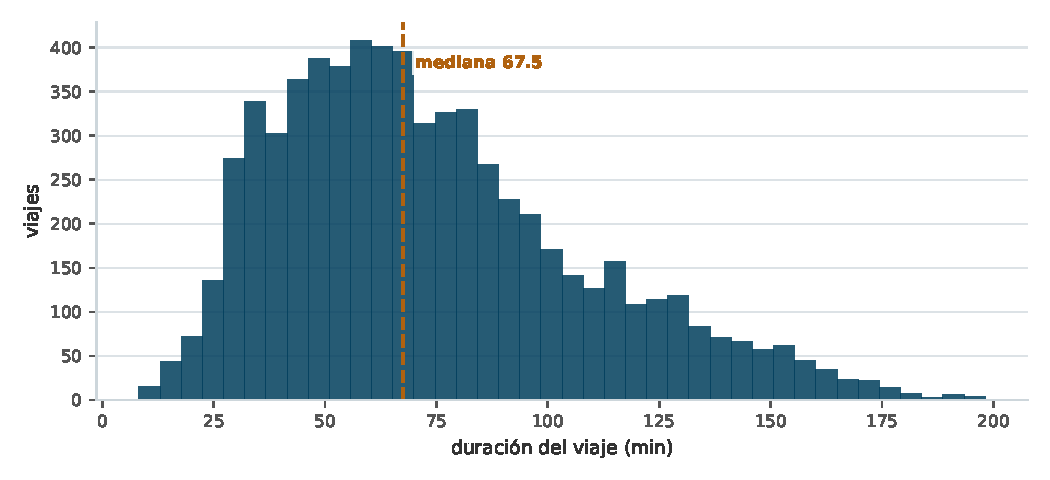
\includegraphics[width=\linewidth]{../03-resultados/fig_duracion.pdf}
\\[5pt]
{\small\itshape\color{slate}Duración de los viajes del día laboral. La cola larga hasta \duracionMax{} min corresponde a recorridos periféricos; son los que más restringen el encadenamiento.}
\end{figure}

\begin{figure}[h]
\centering
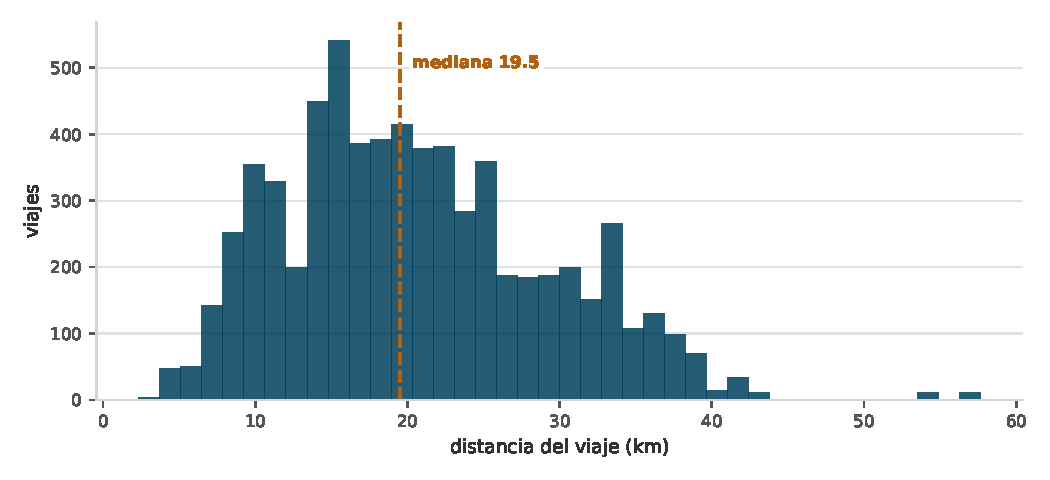
\includegraphics[width=\linewidth]{../03-resultados/fig_distancia.pdf}
\\[5pt]
{\small\itshape\color{slate}Distancia por viaje. Con autonomía útil de \autonomiaUtil{} km, un bus alcanza a encadenar varios viajes medianos antes de tener que recargar, pero los viajes sobre \distanciaMax{} km consumen una fracción alta de la batería en una sola corrida.}
\end{figure}

\clearpage
\section*{3\quad Datos que faltan}
\addcontentsline{toc}{section}{Datos que faltan}

De los \camposDocumentados{} campos que documenta \texttt{parametros\_descripcion.csv}, \textbf{\camposAusentes{} no existen en ningún archivo entregado}:

\begin{nota}
\listaCamposAusentes
\end{nota}

Se agrupan en tres bloques, y cada uno bloquea algo distinto:

\begin{campos}
\item[Tabla de viajes] \texttt{duration\_min}, \texttt{energy\_kwh}, coordenadas de origen y destino, y paraderos inicial y final. Sin ellos no existe la instancia; hay que construirla desde el GTFS crudo.
\item[Deadhead] \texttt{deadhead\_distance\_km}, \texttt{deadhead\_time\_min}, \texttt{pullout\_*} y \texttt{pullin\_*}. Sin ellos no hay costo de desplazamiento vacío, que es la mitad del \textit{trade-off} que plantea el enunciado.
\item[Capacidad de carga] \texttt{num\_chargers}, \texttt{transformer\_mw} y \texttt{max\_charges}. Sin ellos la restricción que el enunciado pone en el centro del problema no se puede escribir.
\end{campos}

\section*{4\quad Verificación de consistencia}
\addcontentsline{toc}{section}{Verificación de consistencia}

\entrada{V1}{La flota declarada no alcanza para la red completa}{\critica}
\begin{campos}
\item[Qué se midió] El máximo de viajes simultáneos del día laboral, que es la cota inferior clásica de flota para un \textit{vehicle scheduling problem}: ningún plan puede usar menos vehículos que viajes solapados haya en el peor instante \citep{bunte_vspoverview_2009}.
\item[Resultado] \textbf{\picoSimultaneo{} viajes simultáneos a las \horaPico}, contra una flota declarada de \flotaDeclarada{} buses en \texttt{parameters.csv}. La red completa exige al menos \ratioFlota$\times$ la flota disponible.
\item[Validación] La cota calculada queda a \desvioValidacion\,\% de la flota real de RED documentada por \citet{galarza_pilotstoscale_2020} para 2018 (\flotaRealRED{} buses). La coincidencia confirma que el GTFS es auténtico y que la expansión de frecuencias está bien hecha.
\item[Implicancia] No es un supuesto que podamos elegir: con \flotaDeclarada{} buses, cubrir la red completa es \textbf{infactible}. O el proyecto trabaja sobre un subconjunto de aproximadamente un quinto de la red, o \texttt{fleet\_size} corresponde a otra cosa.
\end{campos}

\entrada{V2}{Los electroterminales no alcanzan ni para la flota declarada}{\critica}
\begin{campos}
\item[Qué se midió] Suma de \texttt{capacity} sobre los \numElectroterminales{} electroterminales de \texttt{depots.csv}.
\item[Resultado] \textbf{\cuposTotales{} cupos} para una flota declarada de \flotaDeclarada{} buses, y \ratioCupos$\times$ menos que el pico de operación.
\item[Implicancia] Si el modelo exige que cada bus termine el día en un electroterminal, el problema es infactible incluso antes de considerar la energía. El tope real de flota no es \flotaDeclarada{} sino \cuposTotales.
\end{campos}

\entrada{V3}{La restricción de carga simultánea no restringe}{\critica}
\begin{campos}
\item[Qué se midió] Comparación de \campoTT{max\_simultaneous}{charging} y de la columna \texttt{capacity} de \texttt{charging\_activities.csv} contra la capacidad de estacionamiento de cada electroterminal, en los \numElectroterminales{} recintos y en los 24 bloques horarios.
\item[Resultado] Coinciden exactamente en todos los casos, y el valor no varía a lo largo del día. Es decir: todo bus que quepa estacionado puede cargar, simultáneamente, a cualquier hora.
\item[Implicancia] La competencia por los cargadores —el mecanismo que el enunciado describe como fuente de congestión— no está representada en los datos. El archivo entrega la \emph{forma} de la restricción (por electroterminal y por bloque horario) con valores marcadores de posición.
\end{campos}

\entrada{V4}{Los terminales del enunciado no existen en los datos}{\alta}
\begin{campos}
\item[Qué se midió] Búsqueda de menciones a terminales no eléctricos en todos los CSV y en el GTFS.
\item[Resultado] El diccionario define \texttt{depot\_id} exclusivamente como «electroterminal», y \texttt{pullout} y \texttt{pullin} se miden solo contra electroterminal. En el GTFS solo hay paraderos cuyo nombre menciona un terminal, no una instalación modelada aparte.
\item[Implicancia] El enunciado distingue «terminales, electroterminales y puntos de inicio de servicio», tres tipos de nodo. Los datos solo permiten construir dos. Un bus que no necesita cargar no tiene dónde esperar salvo el paradero donde terminó o un electroterminal, lo que infla artificialmente la presión sobre la infraestructura de carga.
\end{campos}

\begin{figure}[h]
\centering
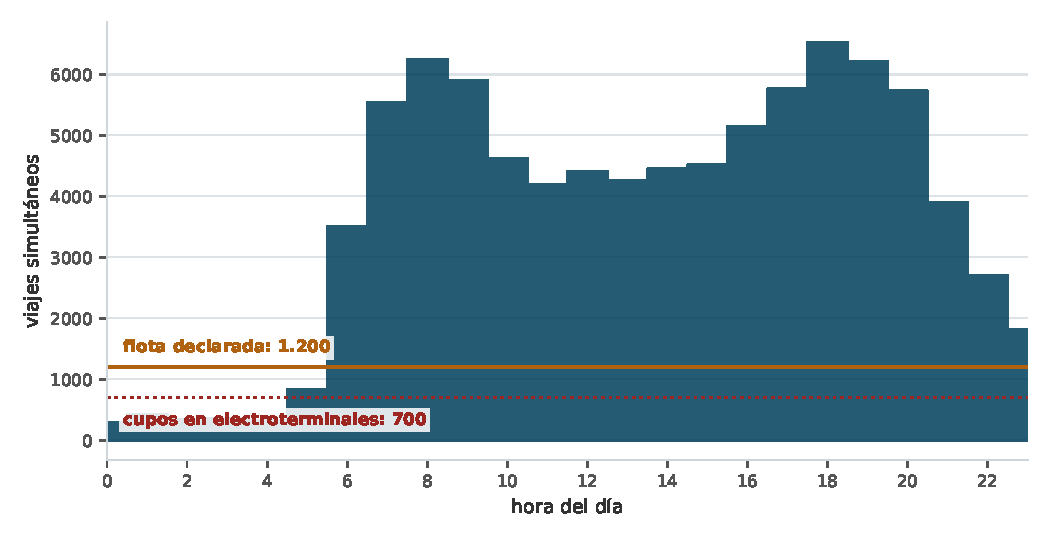
\includegraphics[width=\linewidth]{../03-resultados/fig_concurrencia.pdf}
\\[5pt]
{\small\itshape\color{slate}Viajes simultáneos a lo largo del día laboral, con la flota declarada y los cupos de electroterminal como referencia. Las dos puntas —mañana y tarde— superan por un orden de magnitud los recursos declarados. Este gráfico es el argumento de V1 y V2 en una sola imagen.}
\end{figure}

\clearpage
\section*{5\quad KPIs propuestos}
\addcontentsline{toc}{section}{KPIs propuestos}

\begin{nota}
Separados en tres grupos a propósito. Los de factibilidad no son métricas de desempeño sino requisitos: si alguno falla, el plan no existe y los demás indicadores no significan nada.
\end{nota}

\begin{longtable}{@{}L{1.2cm}L{5.4cm}L{4.4cm}L{4.5cm}@{}}
\rowcolor{headrow}
\thead{} & \thead{Indicador} & \thead{Unidad} & \thead{Por qué está} \\
\endfirsthead
\rowcolor{headrow}
\thead{} & \thead{Indicador} & \thead{Unidad} & \thead{Por qué está} \\
\endhead
\midrule
\multicolumn{4}{@{}l}{\textbf{\textcolor{ink}{Factibilidad}} — binarios; condición de existencia del plan} \\
\midrule
F1 & Cobertura de viajes & \% (debe ser 100) & El enunciado prohíbe omisiones y duplicidades \\
\rowcolor{softrow}
F2 & Violaciones de SoC mínimo & conteo (debe ser 0) & Ningún bus puede quedarse sin carga \\
F3 & Horas-electroterminal sobre capacidad & conteo (debe ser 0) & Restricción de infraestructura \\
\midrule
\multicolumn{4}{@{}l}{\textbf{\textcolor{ink}{Costo}} — todos vienen en USD en \texttt{parameters.csv}, así que son sumables} \\
\midrule
\rowcolor{softrow}
C1 & Costo total de operación & USD/día & Función objetivo candidata \\
C2 & Costo de energía & USD/día & Sensible a \emph{cuándo} se carga \\
\rowcolor{softrow}
C3 & Costo de \textit{deadhead} & USD/día & El otro lado del \textit{trade-off} \\
C4 & Costo fijo de flota & USD/día & Penaliza usar buses de más \\
\rowcolor{softrow}
C5 & Costo de espera & USD/día & Penaliza planes con buses ociosos \\
\midrule
\multicolumn{4}{@{}l}{\textbf{\textcolor{ink}{Uso de recursos}} — explican \emph{por qué} un plan cuesta lo que cuesta} \\
\midrule
U1 & Buses activos vs.\ disponibles & buses y \% & Mide holgura real de flota \\
\rowcolor{softrow}
U2 & Kilómetros muertos sobre totales & \% & Eficiencia del encadenamiento \\
U3 & Recargas por bus por día & conteo & Intensidad de uso de la batería \\
\rowcolor{softrow}
U4 & Ocupación pico por electroterminal & \% de capacidad & Detecta el cuello de botella \\
U5 & Energía comprada en punta vs.\ valle & \% & Conecta el plan con la tarifa horaria; es el que suele quedar fuera \\
\bottomrule
\end{longtable}

\section*{6\quad Qué problema conviene trabajar}
\addcontentsline{toc}{section}{Qué problema conviene trabajar}

Las verificaciones de §4 acotan las opciones más de lo que parece. Con \flotaDeclarada{} buses y \cuposTotales{} cupos, la red completa está fuera de alcance por construcción, no por dificultad computacional.

\begin{longtable}{@{}L{3.3cm}L{3.4cm}L{4.2cm}L{4.6cm}@{}}
\rowcolor{headrow}
\thead{Variante} & \thead{Tamaño} & \thead{Para qué sirve} & \thead{Riesgo} \\
\endfirsthead
\midrule
Instancia pequeña & 1 electroterminal, $\sim$100--500 corridas & Validar la formulación exacta y obtener cotas de optimalidad & Puede ser tan chica que la capacidad de carga nunca se active \\
\addlinespace
\rowcolor{softrow}
Instancia mediana & 1--2 electroterminales, corridas compatibles con \cuposTotales{} cupos & Escenario realista y factible; candidato a caso base del informe & Requiere definir el criterio de recorte y justificarlo \\
\addlinespace
Red completa & \corridasReales{} corridas & Mostrar la escala real del problema & \textbf{Infactible} con la flota e infraestructura entregadas \\
\addlinespace
\rowcolor{softrow}
Con incertidumbre & sobre la instancia mediana & Cierra el vacío que señala \citet{perumal_evspreview_2022} & Multiplica el costo computacional; solo si la determinista ya funciona \\
\bottomrule
\end{longtable}

\begin{nota}
\textbf{\textcolor{ink}{Recomendación.}} Trabajar la instancia mediana como caso base, con la pequeña como banco de pruebas para verificar el modelo exacto contra la heurística. La red completa se reporta como análisis de escala —cuántos buses y cuántos cupos harían falta— en vez de intentar resolverla. Esa cifra ya la tenemos: \picoSimultaneo{} buses en el pico, y es un resultado en sí mismo.
\end{nota}

\clearpage
\renewcommand{\refname}{Referencias citadas}
\bibliography{referencias}

\end{document}
